\documentclass[11pt,a4paper]{report}
\usepackage[latin1]{inputenc}
\usepackage[english]{babel}
\title{General Manual Bebras:\\ Biber}

\usepackage{fullpage}
\usepackage{hyperref}
\usepackage[pdftex]{graphicx}

\setcounter{secnumdepth}{5}
\setcounter{tocdepth}{5}
\makeindex
\begin{document}
\maketitle
\parindent 0pt
\tableofcontents

% Introduction to the manual
\chapter{Introduction}
This is general manual for the Biber version of the Belgian Bebras platform.
 

%General functions
\chapter{General}

\section{Information}
\subsection{Users}
There are four different types of users:\begin{itemize}
\item Pupils can participate in Unrestricted Competitions. If they belong to a class they can also participate in the Official Competitions and Local Competitions.
\item A teacher is responsible for composing his classes, and opening and closing of all competitions for there classes.
\item An organizer is responsible for the creation and uploading of questions, sets, and competitions. 
\item An administrator is the technical manager of the application.
\end{itemize}

\subsection{Competitions}
There are three types of competitions:
\begin{itemize}
\item A Free Competition: This competition can be played by all pupils (with or without class).
\item A Local Competition: Een local competition is created by a teacher, and can only be played by pupils of their classes.
\item An Official Competition: This competition can only be played during the offial bebras week. This competition is only open to classes, and not individual pupils.
\end{itemize}

\subsection{Levels}
The level of a class, and by consequence of all the pupils in the class determines which set from a given competition is available to play. A class can only play sets from the same level as their class level.
\begin{itemize}
\item Ewok: 5th and 6th year grammar school.
\item Wookie: 1st and 2nd high school.
\item Padawan: 3th and 4th high school.
\item Jedi: 5th and 6th high school.
\end{itemize}



\section{General Tasks}

\subsection{Register}
There are a couple of ways to get an account.
\begin{itemize}
\item \textbf {Registration through web application}: You can get registered as a pupil without class. You will get a pupil account but won't be able to play the official competition or any local competitions. You will be able to play all free competitions and see your history. You can register yourself by clicking on the register link on the main page.
\item \textbf{Through teacher}: The best way for a pupil to register is via his participating teacher. This way you can play all competitions if your class participates.
\item \textbf{Different types of accounts}: An administrator can register organizers and an organizer can register teachers. An administrator can only be created by the application manager.
\end{itemize}
With exception of pupils registered by a teacher, everybody gets his login credentials via email. 

\subsection{Login}
You can login through the mainpage of the application by filling in your bebrasID and password. All types of users log in this way. After loggin in, you get redirected to your personal profile page. 
\par
If you log in for the first time, you are obligated to change your temporary password you got by email. The new password needs to be different from the old. This procedure is only needed the first time, other time you will automatically redirected to your personal profile page.

\subsection{Lost or change password?}
When you lost your password or just want to change your password you can click on the reset password link on the main page. On the next page you fill in your bebrasId or your email. You will receive a mail containing a unique link through which you can change your password. This link is only available 1 day. When you are a pupil without an email, you need to ask your teacher to reset your password.

\subsection{Select and change language}
Throughout the application you can change the language at the top left of the page. Current supported languages are: English, Dutch, French and German.

\subsection{Profile page}
When you are logged in you get redirected to your profile page. From here you can access the rest of the application.

\subsection{Edit profile}
Through the link edit profile on your profile page you can at all times change your personal information.  

\subsection{Help page}
At the top right there is a help link. At this page you can find a short summary of how to get to specific actions. 
\subsection{Download userguide}
You can download this manual on your profile page to the left, by clicking on the download manual link. You will only get the part up to your access level.


% Manual for the pupil
\chapter{Pupil}

% A short introduction to what this user can do
\section{Introduction}
Only pupils can participate in competitions. Self registered pupils can participate in Unrestricted Competitions and view their history. If they belong to a class they can also participate in the Official Competitions and Local Competitions. Everybody can register himself as a pupil without class, you don't need to be a real pupil. 
\subsection{Profile page}
On your profile page you can see al the competitions currently available for you. On the right you can see a link for viewing your history.
\subsection{View history}
After playing a competition, you can always find back your results by going to your history page. On this page you will see a list of all played competitions.

\section{Participating in competition}
\subsection{Before}
To participate in a competition, you click on an available competition on your profile page. You will see the start screen of the competition. Here you see the general information of the competition, like how much time you have to finish it. If you click on 'start competition' the competition will start.
\subsection{During}
Once the competition is underway, you will get to see the questions. There are two kinds of questions:
\begin{itemize}
\item \textbf{Multiple Choice}: You simply click on an answer (A, B, C or D). You will immediately get directed to the next question. 
\item \textbf{Open questions}: For this type of question you need to enter a number, word or short sentence in the text field and click on submit.
\end{itemize}
Each time you answered a question, you will be directed to the next question. It is possible to return later to a previous question by clicking on the right question on the right side of the screen.
\subsection{After}
If you are ready with the competition, you click on 'finish competition'. If you have participated in a Local or Unrestricted competition you will see a feedback page where you can see your results and click on questions for feedback. 

\begin{figure}[h!]
\centering
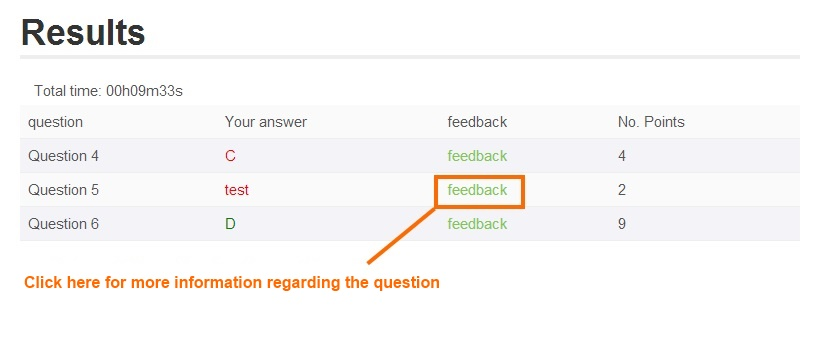
\includegraphics[width=\textwidth]{results_en.jpg}
\caption{Screen after finishing a competition. Here you can find all your answers and view feedback for some questions.}
\label{fig:results}
\end{figure}

\subsection{Statistics of Competition}
When you go to your history and select a competition, you can see how you did compared to the rest of the pupils by clicking on the statistics link. 

\section{Official Competition}
This is an annual competition, en is similar to the other types of competitions. The only real difference is that after finishing you will not immediately see your results. A teacher needs to open this competition for the class.
\begin{itemize}
  \item \textbf{Paticipating}: U can only participate if you are part of a class, and this class participates in the competition. This is the responsibiliy of the teacher, encourage him to participate if he isn't already participating.
	\item \textbf{Resultaten}:  The results of the official competition are only visible after the competition is closed for all classes, normally one week after the start. U can view the results by checking your history or asking your teacher.
\end{itemize}


% Manual for the teacher
\chapter{Teacher}

%Section
\section{Introduction}
A teacher registers himself by sending an email with his personal information to an organizer. He also needs to send the information of all the schools where he wants to have participating classes. After registration a teacher is responsible for creating classes and registering pupils to this classes. He can create and open local competitions and let his classes participate in the official competition.

\subsection{Profile page}
You can find your classes, your local competition en if there any, the official competitions on your profile page.
%Sectie
\section{Competitions}
As a teacher you can create local competitions for a class, this puts you in the position to prepare your class for the official competition.
\subsection{Lokale competitie}
\subsubsection{Create}
First you need to create a local competition. You do this by clicking on the link 'New local competition' on your profilepage. You need to give for each language you want a title (minimum one language). After that you can add maximum one set for each level. Think of the fact that classes can only play sets which are of the same level as the general class level.
\subsubsection{Open}
After creating, the competition will appear on your profile page. When u click on the competition, you will find a page where you can open this competition for one or more of your classes. Those classes will be able to play the local competition.

\subsubsection{Closing and Results}
If you want to download the results of a class, you need to close the competition for this class. You can do this by clicking on the red cross next to the competition on your profile page and select the classes for who you want to close the competition. When you did this, nobody of those classes will be able to play the competition. Now you can download the results by first going to the class page for the particular class. This you do by clicing on the class on your profilepage. On the next page you will on the right side a link 'View Recent Competitions', where you need to click on. Now you will see all the closed competitions for this class and can you download the results in an appropriate file format, each download button represents a different file download format. 

\subsubsection{Monitor Pupils}
During a competition you can monitor your students. If you click on the competition on your profile page after you opened the competition you will find the possibility to monitor. When clicking on this link, you will find an overview of all your pupils who should be participating in the competition. For each individual pupil you can do the following actions:
\begin{itemize}
	\item Give additional time: With this button you can give a pupil additional time to finish the competition. The format is hours:minutes:seconds.
	\item Delete history: With this action you can delete the entire question history of a pupil for this specific competition, and will remove the participation of the pupil. This will have as consequence that a pupil can retake the competition, and that none of his previous answers have been stored.
	\item Reopen competition: With this function you can reopen a competition for a pupil, after the competition is finished for this particular pupil.  His answers stay visible. How much time he gets you need to decide yourself through the format hour:minutes:seconds.
\end{itemize}

\begin{figure}[h!]
\centering
\includegraphics[width=\textwidth]{monitor_en.jpg}
\caption{Screen for monitoring pupils during competition.}
\label{fig:monitor}
\end{figure}


\subsection{Official Competition}
The official competitions takes place during a preselected week. In this week you will find under your competitions on your profile page an extra competition, recognizable by an extra star. You need to open en close this competition for each of your classes. You do this best just before your class starts with the competition.

%Sectie
\section{Classes and Pupils}
\subsection{Add class}
You can add a class by simply clicking on the green add symbol on your profile page under 'My Classes'. You will see a pop-up screen where you need to fill in the school, level and name of the class. In case the school of the class isn't in the system, you need to contact an organizer in an email with the information of the school, so he can add the school.

\subsection{Class page}
When clicking on the name of the class on your profile page you will go to his class page. There you can find an overview of all the pupils registered with this class, and you can see if they are online. If the circle before the name is red, the pupil is offline, if the circle is green, the person is online. You can do the following functions on this page:

\subsubsection{Reset password pupil}
When one of your pupils has lost his or her password, you can reset this password. Next to each pupil there is a reset button, when you click this button, you will receive an email containing an new (temporary) password for the pupil. The pupil can log in with the new password, and will immediately be requested to change his temporary password to a personal password.

\subsubsection{Add existing pupils to class}
If you want to register pupils who are already in the system, you can do this easily by clicking on the green add button at the bottom. In the pop up screen you fill in the bebrasId of the existing pupil. The pupil will be immediately added to the class list.
\subsubsection{Add single pupil to class}
When you are on the class page, you will find in the list of links on the right side a link to add a single pupil to the class. You need to fill in the form, all fiels are required except the email field. After registering you will receive an email containing the pupil's login credentials.
\subsection{Add multiple pupiles and multiple classes}
On your profilepage to the left, you can find a link 'Register Pupils' where you can upload a file containing the data of pupils. You can add one or more new or existing pupils. You can also simultaneously register multiple classes, but they all have to belong to the same school. The easiest way to fulfill to the requiered format is to download a sample in the requiered format. There are three file formats available: xls (excell 1997-2003), xlsx (excell 2007-current) and csv.
\subsubsection{Excell}
This are the specifications for both the xls and xlsx format. The title of each sheet decides the name of the class (see figure).  If the class already exists in the school and you are responsible for the class, the pupils will be added to the class. If the uploaded document doesn't fulfill the requiered specifications, you will be noticed, and you will need to change the document and upload it again.
\\ \textbf{Specifications}:
\begin{itemize}
\item Row 1: Beginyear of the current schoolyear. For the schoolyear 2002-2003 you should fill in 2002.
\item Row 2: Level of the class. Choices: EWOK, WOOKIE, PADAWAN or JEDI.
\item Row 3: Nothing requiered. To make it yourself easier, you can fill in here the column names in the following order: First Name, Last Name, E-mail (optional), Gender, Language, Birth date (dd/mm/yyyy), BebrasId. This last field only is needed when the pupil is already registered in the system. When you download a sample, this fields will be added automatically.
\item Starting from row 4 all the information of the pupils needs to be entered.
\end{itemize}
\subsubsection{Csv}
Entering information into a csv document is similar to the specifications used for excell. Instead of using sheets for different classes you only need to leave a line blank. For more details please download an example.
\subsubsection{Handling}
If everything is correct when uploading, you will get an email containing a attachment in the same file format as the requested format. The file contains login credentials for all newly registered pupils. If you registered an already exisiting pupil by filling in the correct bebrasId in the requiered field, there will be no password, because the old password will still be valid. The new or updated classes will be visible on your profile page.
\begin{figure}[h!]
\centering
\includegraphics[width=\textwidth]{uploadPupils_en.jpg}
\caption{Example of excell file to register pupils.}
\label{fig:uploadPupils}
\end{figure}

\subsection{Download classes from a school}
Via the 'download classes' link on your profilepage you can download all classes of your current schools in an appropriate file format (excell xlsx, excell xls, csv). You can choose between the registered classes of this year or the registered classes of the previous year. This can be usefull when needing to register pupils in the beginning of the new year, when most of them have already participated last year, and are still in the same school.

\subsection{Merging Pupils}
When u click on the link 'Merge Pupils' on your profile page, you can merge pupils from your schools who have accidentally registered themselves twice. You need to search on the name of the pupil. You will get an overview of all bebrasId's who are created under this name in your schools. You have to select all the profiles of the specific pupil. These profiles will show up in the list underneath. Of those profiles you select one to keep, the others will be deleted. The history of those accounts will be transfered to the survivor account. 

\subsection{Download statistics of pupils}
You can download basic competition statistics of the pupils in different ways. You can see individual stats while monitoring the students. Or you can see global stats after finishing the competition via the link on the class page.


% Manual for the organiser
\chapter{Organizer}

%Sectie
\section{Introduction}
An organizer primarily needs to manage the application. He is responsible for the registering of teachers and schools. He has the important tasks of ending the schoolyear. He is also the only type of user who can upload questions and create unrestricted competitions. He needs to make, create, open and close the official competition.

%Sectie
\section{Schools and teachers}
An organizer creates teachers and there respective schools. Once a teacher and his school are in the system, the teacher himself is responsible to create classes and add pupils to his classes. 
\subsection{Register school and teacher}
When you want to register a teacher you need his personal details, and the details of all the schools where the teacher wants participating classes. This details are best received by email. Once you have this information, you first need to check if the school(s) are already in the system. If this is not the case, you need to register the schools. You can do this by clicking the 'register school' link on your profile page. Here you enter the details of the schools, who will enters the system immediately. After this, you can register the teacher via the 'register teacher' link on your profile page. On the next page you enter all required fields and select the schools corresponding to the teacher. After registration, the teacher will receive his login credentials by email.

\subsection{Taking over teacher account}
You can temporarily take over a teacher account by clicking on the top right of your profile page on 'Mimick User' link. In the pop up screen you enter the bebrasId of the teacher you want to be. After you submitted you will be redirected to the teacher his profile page. Now you are logged in as the specified teacher and you can do all functions the teacher would be able to. When you are finished you click on the log out link, you will be redirected to your own profile page. 

\subsection{Finishing a Schoolyear}
At the end of the schoolyear, it is necessary that an organizer discontinues the current classes. You can do this by clicking the 'end schoolyear' link on your profile page. Read the instructions carefully and submit. This will disconnects all pupils and teachers of their current classes. This should preferably happen between the 1st July and 31th August. This action cannot be undone, be carefull.  

%Sectie
\section{Questions, Sets and Competitions}
Organizers have the task to upload the questions to the application, to select the questions on the basis of difficulty to create a set, and to form a competition with sets for each age category.

\subsection{Create or Edit Questions}
When clicking on 'upload new question' you will get the choice between uploading existing html pages to the application in a zip file or create or edit a question with the build in 'what you see is what you get' editor.

\subsubsection{Upload zip file}
For this method you need to add all your question (html file)/feedback (html file)/image files of all the questions you want to add to a zip container and upload it to the application. If there are errors you wil get noticed. When succesfull you will go to the next screen. Here you first need to specify if you want to add a new question or choose an existing question from the database to edit. After that you choose for which language you want to add/edit the question. The next step is choosing the correct question file and if necessary a feedback page. At the top you need to specify the answer. There are two possible answer methods. Multiple choice (A, B, C or D) or regular expression, where you can input any text or numbers you want. After that you can submit the question to the database.

\subsubsection{With wysiwyg editor}
This method is similar to the method above, but you don't need to upload any html files to the application. You will simply write your questions in a word like editor right in the application itself.  Instead of choosing the file to upload you type your question in the question editor, or your feedback in the feedback editor. The two editors are at the bottom of the page.
\begin{figure}[h!]
\centering
\includegraphics[width=\textwidth]{uploadQuestion_en.jpg}
\caption{Screen to upload or edit questions.}
\label{fig:uploadQuestion}
\end{figure}

\subsection{Create a question set}
To bundle the question to a set you need to do the following. You click on the 'create question set' link on your profile page. You need to do two things.
\begin{itemize}
\item \textbf{General information}: At the top of the page you have to click on 'choose information' to show the form where you need to enter the details of the set. You need to enter a \textbf{title} in at least one language. You also need to enter a\textbf{ time limit} in minutes. The \textbf{public} of a set determines which competitions can use this set. Official can only be used for the official competition. Local competitions can only be used by teachers for making local competitions. Unrestricted sets will create an unrestricted competition, the moment they are set visible.  The \textbf{visibility} of a set determines if other people than organizers can see the competition, and if it can already be used to create competitions. The level of the set determines which classes will play this set, because only classes with the same level as the set can that set.

\item \textbf{Selecting questions}: You see a list with all available questions, between brackets are the available languages of the question. To add a question to the set, click the checkbox before the question. Now there will appear three input fields. First you have to select the difficulty of the question, second you need to enter how many points pupils will receive when they answer the question correct, and last you need to enter the points that will get deducted when they answer wrong. Both numbers need to be positive.
\end{itemize}
To the right you can find the list of already selected questions. When you want to save the set, click the 'create' button.

\begin{figure}[h!]
\centering
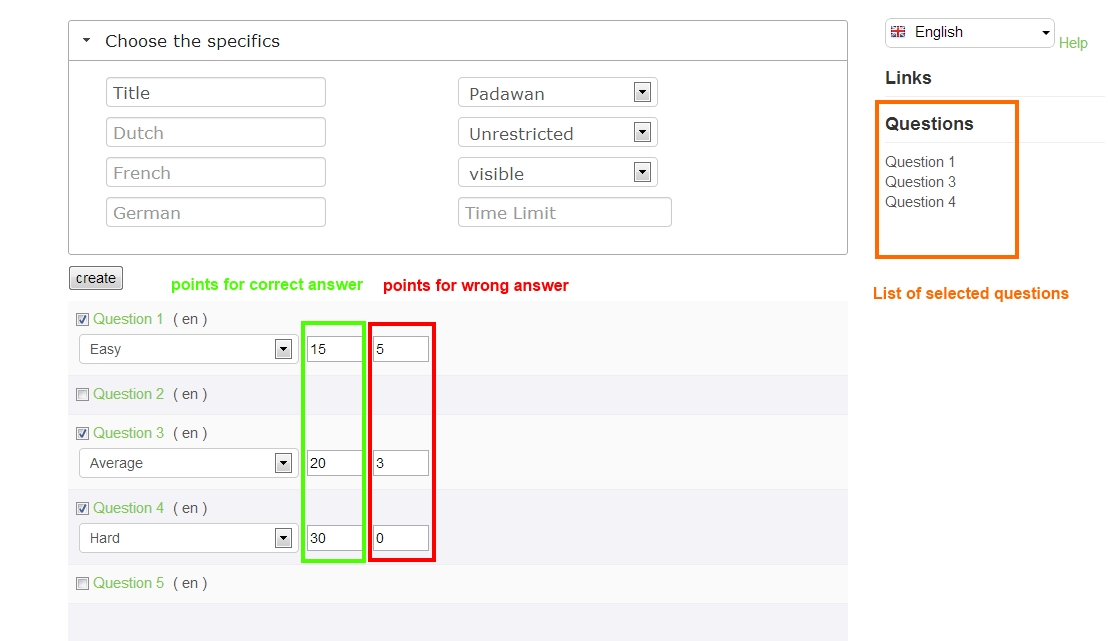
\includegraphics[width=\textwidth]{makesets_en.jpg}
\caption{Screen for creating question sets.}
\label{fig:makesets}
\end{figure}

\subsection{Manage question sets}
On this page you can, accessible through your profile page, you can delete, add en edit sets. To simply change the visibility, you can click on the arrows next to the set. Those will raise or decrease the visibility. To add, remove or edit other details, click on the appropriate buttons next to the set.

\subsection{Create competition}
\textbf{Unrestricted Competition}: An unrestricted competition is automatically created when you create a question set of the type unrestricted, with open visibility.
\\ \\
\textbf{Official competition}: This is created the following way. Click the link 'create new competition' to the right of your profile page. You need to do two things.
\begin{itemize}
		\item \textbf{Give name}: At least one language should have a title 
		\item \textbf{Select sets}: For each level you can choose maximum one set. All sets of the type official will be available to choose.  
\end{itemize}

\subsection{Open competitions}
On your profile page you can see a list of competitions you have created. The lock next to each competition shows if the competition is open or closed.

\subsection{Statistics}
You can find statistics for each set on the 'manage sets' page.

% Manual for the admin
\chapter{Admin}

\section{Introduction}
An administrator accounts get created by the application developper. The most important task of the admin is the registering of organizers and the managing of the ftp servers. 
\section{Register Organizer}
Via the link 'Register Organizer' on your profilepage, you will get to the registrationpage. This page will show a form where you can enter the details the details of the organizer. All fields are requiered. After registration, you will receive an email containing the login credetials of the newly registered organizer.

\section{Taking over Teacher/Organizer Account}
An admin is able to take over the account of a teacher or organizer. This happens the same way a organizer mimics teachers. You need to click on the top right of your profile page on the 'Mimick User'. Here you fill in the bebrasId of the requested account. Now you are logged in as that person.
\section{Managing FTP Servers}
If you click on the manage ftp servers' on your profile page, you will be directed to a page where you have an overview of the current ftp servers. On this page you add, delete and edit servers.
\begin{itemize} 
	\item Add server: Click on the button at the bottom right. You will see a form where you need to fill in the requiered details.
	\item Edit server: Click in the overview on the pencil next to the server you want to edit. You will see a page where you can edit the details of the server.
	\item Delete server: Click in the overview on the delete icon next to the server. This server will be deleted from the system.
\end{itemize}

\begin{figure}[h!]
\centering
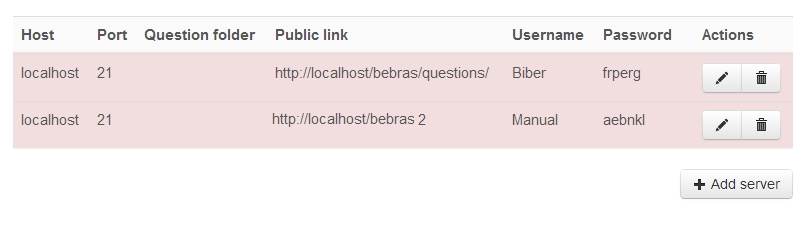
\includegraphics[width=\textwidth]{manageftp_en.jpg}
\caption{Screen for managing of ftp servers: here you can add, delete and edit servers.}
\label{fig:manageftp}
\end{figure}


\end{document}